%%%%%%%%%%%%%%%%%%%%%%%%%%%%%%%%%%%
%This is the LaTeX COMMUNICATION template for RSC journals
%Copyright The Royal Society of Chemistry 2016
%%%%%%%%%%%%%%%%%%%%%%%%%%%%%%%%%%%

\documentclass[twoside,twocolumn,9pt]{article}
\usepackage{extsizes}
\usepackage[super,sort&compress,comma]{natbib} 
\usepackage[version=3]{mhchem}
\usepackage[left=1.5cm, right=1.5cm, top=1.785cm, bottom=2.0cm]{geometry}
\usepackage{balance}
\usepackage{mathptmx}
\usepackage{sectsty}
\usepackage{graphicx} 
\usepackage{lastpage}
\usepackage[format=plain,justification=justified,singlelinecheck=false,font={stretch=1.125,small,sf},labelfont=bf,labelsep=space]{caption}
\usepackage{float}
\usepackage{fancyhdr}
\usepackage{fnpos}
\usepackage[english]{babel}
\addto{\captionsenglish}{%
  \renewcommand{\refname}{Notes and references}
}
\usepackage{array}
\usepackage{droidsans}
\usepackage{charter}
\usepackage[T1]{fontenc}
\usepackage[usenames,dvipsnames]{xcolor}
\usepackage{setspace}
\usepackage[compact]{titlesec}
\usepackage{hyperref}
%%%Please don't disable any packages in the preamble, as this may cause the template to display incorrectly.%%%


\usepackage{epstopdf}%This line makes .eps figures into .pdf - please comment out if not required.
\usepackage{multirow}

\definecolor{cream}{RGB}{222,217,201}
\begin{document}

\pagestyle{fancy}
\thispagestyle{plain}
\fancypagestyle{plain}{
%%%HEADER%%%
\renewcommand{\headrulewidth}{0pt}
}
%%%END OF HEADER%%%

%%%PAGE SETUP - Please do not change any commands within this section%%%
\makeFNbottom
\makeatletter
\renewcommand\LARGE{\@setfontsize\LARGE{15pt}{17}}
\renewcommand\Large{\@setfontsize\Large{12pt}{14}}
\renewcommand\large{\@setfontsize\large{10pt}{12}}
\renewcommand\footnotesize{\@setfontsize\footnotesize{7pt}{10}}
\renewcommand\scriptsize{\@setfontsize\scriptsize{7pt}{7}}
\makeatother

\renewcommand{\thefootnote}{\fnsymbol{footnote}}
\renewcommand\footnoterule{\vspace*{1pt}% 
\color{cream}\hrule width 3.5in height 0.4pt \color{black} \vspace*{5pt}} 
\setcounter{secnumdepth}{5}

\makeatletter 
\renewcommand\@biblabel[1]{#1}            
\renewcommand\@makefntext[1]% 
{\noindent\makebox[0pt][r]{\@thefnmark\,}#1}
\makeatother 
\renewcommand{\figurename}{\small{Fig.}~}
\sectionfont{\sffamily\Large}
\subsectionfont{\normalsize}
\subsubsectionfont{\bf}
\setstretch{1.125} %In particular, please do not alter this line.
\setlength{\skip\footins}{0.8cm}
\setlength{\footnotesep}{0.25cm}
\setlength{\jot}{10pt}
\titlespacing*{\section}{0pt}{4pt}{4pt}
\titlespacing*{\subsection}{0pt}{15pt}{1pt}
%%%END OF PAGE SETUP%%%

%%%FOOTER%%%
\fancyfoot{}
\fancyfoot[LO,RE]{\vspace{-7.1pt}
\includegraphics[height=9pt]{head_foot/LF}}
\fancyfoot[CO]{\vspace{-7.1pt}\hspace{13.2cm}
\includegraphics{head_foot/RF}}
\fancyfoot[CE]{\vspace{-7.2pt}\hspace{-14.2cm}
\includegraphics{head_foot/RF}}
\fancyfoot[RO]{\footnotesize{\sffamily{1--\pageref{LastPage} ~\textbar  \hspace{2pt}\thepage}}}
\fancyfoot[LE]{\footnotesize{\sffamily{\thepage~\textbar\hspace{3.45cm} 1--\pageref{LastPage}}}}
\fancyhead{}
\renewcommand{\headrulewidth}{0pt} 
\renewcommand{\footrulewidth}{0pt}
\setlength{\arrayrulewidth}{1pt}
\setlength{\columnsep}{6.5mm}
\setlength\bibsep{1pt}
%%%END OF FOOTER%%%

%%%FIGURE SETUP - please do not change any commands within this section%%%
\makeatletter 
\newlength{\figrulesep} 
\setlength{\figrulesep}{0.5\textfloatsep} 

\newcommand{\topfigrule}{\vspace*{-1pt}% 
\noindent{\color{cream}\rule[-\figrulesep]{\columnwidth}{1.5pt}} }

\newcommand{\botfigrule}{\vspace*{-2pt}% 
\noindent{\color{cream}\rule[\figrulesep]{\columnwidth}{1.5pt}} }

\newcommand{\dblfigrule}{\vspace*{-1pt}% 
\noindent{\color{cream}\rule[-\figrulesep]{\textwidth}{1.5pt}} }

\makeatother
%%%END OF FIGURE SETUP%%%

%%%TITLE AND AUTHORS%%%
\twocolumn[
  \begin{@twocolumnfalse}
{
\includegraphics[height=30pt]{head_foot/journal_name}\hfill\raisebox{0pt}[0pt][0pt]{
\includegraphics[height=55pt]{head_foot/RSC_LOGO_CMYK}}\\[1ex]

\includegraphics[width=18.5cm]{head_foot/header_bar}}\par
\vspace{1em}
\sffamily
\begin{tabular}{m{4.5cm} p{13.5cm} }


\includegraphics{head_foot/DOI} & \noindent\LARGE{\textbf{A Green, Reagent-Saving Analytical Strategy for Equivalence Point Determination in Potentiometric Titrations via Gran and Schwartz Linerarisation}} \\%Article title goes here instead of the text "This is the title
 & \vspace{0.3cm} \\

 & \noindent\large{Samuele Giani,$^{\ast}$\textit{$^{a}$} and Cosimo A. De Caro,$^{\ast}$\textit{$^{b}$}} \\%Author names go here instead of "Full name", etc.

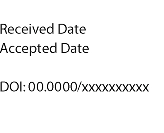
\includegraphics{head_foot/dates} & \\

\end{tabular}

 \end{@twocolumnfalse} \vspace{0.6cm}

  ]
%%%END OF TITLE AND AUTHORS%%%

%%%FONT SETUP - please do not change any commands within this section
\renewcommand*\rmdefault{bch}\normalfont\upshape
\rmfamily
\section*{}
\vspace{-1cm}


%%%FOOTNOTES%%%

\footnotetext{\textit{$^{a}$~Universitätsspital Zürich, Rämistrasse 100, 8091 Zürich, Switzerland. E-mail: samuele.giani@usz.ch}}
\footnotetext{\textit{$^{b}$~Mettler-Toledo Technologies GmbH, Heuwinkelstrasse 3, 8606 Nänikon, Switzerland. E-mail: cosimo.decaro@mt.com}}

%Please use \dag to cite the ESI in the main text of the article.
%If you article does not have ESI please remove the the \dag symbol from the title and the footnotetext below.

%%% \footnotetext{\dag~Supplementary Information available: Access Links, detailed equations derivation and analytical workflow. See DOI: 00.0000/00000000.}

%additional addresses can be cited as above using the lower-case letters, c, d, e... If all authors are from the same address, no letter is required

%\footnotetext{\dag~Additional footnotes to the title and authors can be included \textit{e.g.}\ `Present address:' or `These authors contributed equally to this work' as above using the symbols: \ddag, \textsection, and \P. Please place the appropriate symbol next to the author's name and include a \texttt{\textbackslash footnotetext} entry in the the correct place in the list.}

%%%END OF FOOTNOTES%%%

%%%ABSTRACT%%%%

\sffamily{\textbf{
%
Potentiometric titrations remain a cornerstone of analytical chemistry, yet conventional methods require titration well beyond the equivalence point, generating unnecessary chemical waste.
Here we introduce a sustainable two-stage analytical strategy based on Gran and Schwartz linerarisation methods for equivalence point determination with significantly reduced reagent consumption. 
%
In the first stage, a usual titration is performed past the equivalence point to determine a reliable reference equivalence point (EQP*, full curve).
In the second stage, systematic backward trimming of the same dataset combined with Gran--Schwartz linerarisation identifies the earliest acceptable volume ($V_{\rm opt}$) at which the Gran--Schwartz equivalence point (EQP, shorten curve) converges within a defined accuracy threshold.
This optimised volume is systematically smaller than both the full titration volume used and the EQP* volume as well, enabling direct reagent savings.
%
The strategy was validated on two benchmark aqueous systems: \ce{TRIS}/\ce{HCl} (weak base--strong acid) and \ce{KHP}/\ce{NaOH} (weak acid--strong base).
Depending on the chosen accuracy threshold, e.g. 0.010--0.050\,mL, reagent savings of approximately 10--30\,\% per titration were achieved while maintaining excellent agreement with the reference EQP* on replicated determinations.
These results directly support Green Chemistry Principle 1 (prevention of waste) and Principle 5 (safer solvents and auxiliaries) by reducing titrant consumption and laboratory waste without compromising analytical accuracy, precision or reliability.
%
Implemented in the open-source Python tool \textsf{GranTED}, this analytical strategy is freely available, providing an accessible, reproducible, and sustainable platform for both research, quality control and teaching laboratories.}}

%%%END OF ABSTRACT%%%%

\rmfamily %Please do not remove this line.

%%%MAIN TEXT%%%%

\section*{Introduction}

Potentiometric titrations are among the most widely used analytical techniques in both research, quality control and teaching laboratories for accurate content determination of specific analytes present in samples by means of chemical reactions such as acid--base neutralization, redox, complexation and precipitation.
Conventional procedures typically require titration well beyond the equivalence point (post-EQP, full-curve) to reliably identify the inflection point, most notably via derivative analysis.
This practice leads to unnecessary consumption of titrant and generates avoidable chemical waste, conflicting with core principles of Green Chemistry.\cite{Anastas1998}

Classical linerarisation methods, first introduced by Gunnar Gran in 1950--1952\,\cite{Gran1950,Gran1952} and later extended by Schwartz in 1987\,\cite{Schwartz1987}, offer a powerful alternative by transforming the sigmoidal titration curve into straight lines whose intersection to the volume axis directly yields the equivalence point.
These approaches can provide higher accuracy and precision than traditional derivative methods, particularly for weak acid--base chemical systems, as well as for poorly detectable endpoints.
However, their practical implementation has largely remained manual, requiring full titration datasets and subjective selection of the linear region.\cite{Macc1989, MICHALOWSKI2005, Martin}

Here we introduce the analytical strategy \textsf{GranTED} (Gran Titration Equivalence point Determination), available as an open-source Python toolkit at \href{https://github.com/sgiani95/GranTED/}{\texttt{https://github.com/sgiani95/GranTED/}}, that fully automates Gran and Schwartz linerarisation while incorporating a novel two-stage optimisation approach.
In the first stage, a complete titration past the equivalence point establishes a reference equivalence point (EQP*).
In the second stage, systematic backward trimming of the same dataset identifies the earliest acceptable volume (\(V_{\rm opt}\)) at which the Gran--Schwartz equivalence point (EQP) diverges from EQP* within a user-defined accuracy threshold.
This optimised volume is systematically smaller than both the full titration volume and the volume at EQP*, enabling direct reagent savings without additional experiments or loss of analytical quality.

The performance of this strategy was rigorously evaluated on two standard benchmark aqueous systems: \ce{TRIS}/\ce{HCl} (weak base--strong acid) and \ce{KHP}/\ce{NaOH} (weak acid--strong base). By combining automated linear-region detection, convergence diagnostics, and quantitative trimming analysis, \textsf{GranTED} transforms a classical analytical procedure into a greener, more efficient, repeatable and reproducible method.
This work demonstrates how modern computational tools can reduce laboratory waste while maintaining analytical reliability, in full alignment with Green Chemistry principles.

\section*{Experimental}

\subsection*{Materials and Instrumentation}

All titrations were performed using analytical-grade reagents.
Tris(hydroxymethyl)aminomethane (\ce{TRIS},99.97\,\%) and potassium hydrogen phthalate (\ce{KHP}, 99.92\,\% ) were obtained from Merck Sigma-Aldrich and used as received.
0.1\,M aqueous solution has been prepared by first dissolving accurately weighed 0.1\,mol of each substances in 500\,mL ultra-pure water (18.2\,M$\Omega\,\cdot\,{\rm cm}$). Subsequently, the solution was added into a 1000\,mL volumetric flask and filled up to the mark with deionised water, respectively. Hydrochloric acid (0.1\,M HCl, Titripac) and sodium hydroxide (0.1\,M NaOH, Titripac) solutions were purchased from Merck Millipore and used without additional preparation. 

Potentiometric measurements were carried out with a Mettler-Toledo T5 automatic titrator equipped with a DGi111-SC combined pH glass electrode.
All experiments were conducted at room temperature under stirring (1000\,rpm). Data were recorded as potential $E$ (mV) versus volume $V$ (mL). % giving a E-V graphical representation of the titration curve.

\subsection*{Titration Protocols}

Two aqueous solution standard benchmark systems were investigated: (i) \ce{TRIS}/\ce{HCl} (weak base–-strong acid) and (ii) \ce{KHP}/\ce{NaOH} (weak acid–-strong base).

A 100\,mL titration beaker was filled with 60\,mL ultra-pure water, and connected to the titration stand of the automatic titrator. The titration method was started, and 5\,mL 0.1\,M TRIS (or KHP) solution was automatically added by a 10\,mL piston-motorised burette before starting the titration. Subsequently, the titrant addition was performed with a 10\,mL piston motorised burette (0.001\,mL resolution), using fixed 0.05\,mL increments.
In both cases, the titration was continued well past the equivalence point %(typically to 120–150\,\% of the expected equivalence volume)
to generate the complete dataset required for reference EQP* determination.% This is automatically achieved by built-in first derivative evaluation procedure in the titrator.
Finally, each system was analysed in sextuplicate to collect enough data for statistical comparison.

\subsection*{Data Analysis with GranTED}

All raw titration data (potential vs.\, volume) previously obtained as described by automated titration were subsequently processed using the developed open-source Python toolkit \textsf{GranTED} (version 2.0.21). The software automatically converts potential to pH, computes both Gran (\,\(g_1\, =\, V\,\cdot\,10^{\;{\rm -pH}}\)\,) and Schwartz (\mbox{\,\(g_s\, =\, (V+k)\,\cdot\,10^{\;{\rm -pH}}\)}\,) functions (\,\(V\)= the dispensed reagent volume, \(k\) = optimisation parameter), identifies optimal linear regions via derivative-based segmentation and R$^2$ maximisation, and performs the backward trimming analysis at the core of the algorithm. User-defined parameters were different EQP deviation threshold 0.010\,mL, 0.020\,mL and 0.050\,mL. All calculations and reporting were performed on a standard laptop in few seconds (Python 3.14 environment).

\section*{Results and Discussion}

\subsection*{Method Development: Earliest Acceptable Volume and Gran--Schwartz optimisation}

The key innovation of the analytical strategy is a two-stage procedure that combines classical Gran and Schwartz linerarisation with systematic backward data trimming to identify the earliest volume at which a reliable equivalence point can be obtained. 

In the first stage, a conventional full titration is performed well past the equivalence point.
The complete dataset is processed with the automated Gran--Schwartz algorithm to determine a high-confidence reference equivalence point, denoted EQP*.
This value serves as the benchmark for subsequent optimisation.

In the second stage, the same experimental dataset is subjected to iterative backward trimming.
Starting from the full titration and progressively removing data points from the post-EQP* region, the Gran--Schwartz linerarisation is reapplied at each step.
For each trimmed dataset, the Gran--Schwartz equivalence point, EQP, is calculated and compared to the reference EQP*.
The difference $|\text{EQP} - \text{EQP*}|$ is evaluated.

The earliest volume, at which the Gran--Schwartz EQP diverges and remains outside the chosen threshold for a number of consecutive points, is defined as the optimised volume, $V_{\rm opt}$.
The value $V_{\rm opt}$ is systematically smaller than both the total titration volume as well as the volume corresponding to EQP*, while still delivering an equivalence point of acceptable accuracy and precision.

Figure~\ref{fig:titrations} a) shows a representative titration curve obtained by titration of the moderately weak base TRIS (\({\rm p}K_{b}({\rm TRIS}) \approx 5.9\)) with the strong acid \ce{HCl}. Note that the sigmoidal pH--$V$ curve shows the expected profile of such a system.

Figure~\ref{fig:titrations} b) shows the corresponding Gran--Schwartz plot for the full dataset of Figure~\ref{fig:titrations} a), where the pre-equivalence point region was successfully linearised between approx. 2.3 and 5\,mL. This is in agreement with Gran's theory for transforming curved profiles into straight lines, furthermore enhanced by electroneutrality compensations to account for [\ce{H+}] dominance (or [\ce{OH-}], respectively), as described by Schwartz.

In Figure~\ref{fig:titrations} c) and d) the trimmed dataset are given for $V_{\rm opt}$ = 4.4\,mL. Note that the shaded, linear segment spans a range between approx. 2.1 and 4.4 mL. 

A convergence table (Table~\ref{tab:trimming}) illustrates how Gran--Schwartz EQP, its uncertainty, the coefficient of determination R$^2$ and the difference $\text{EQP} - \text{EQP*}$ evolve with the number of retained data points, clearly identifying the earliest acceptable volume, as a function of the accuracy threshold (e.g. 0.010--0.050\,mL) defined by the user. 

\begin{figure*}[h]
\centering
  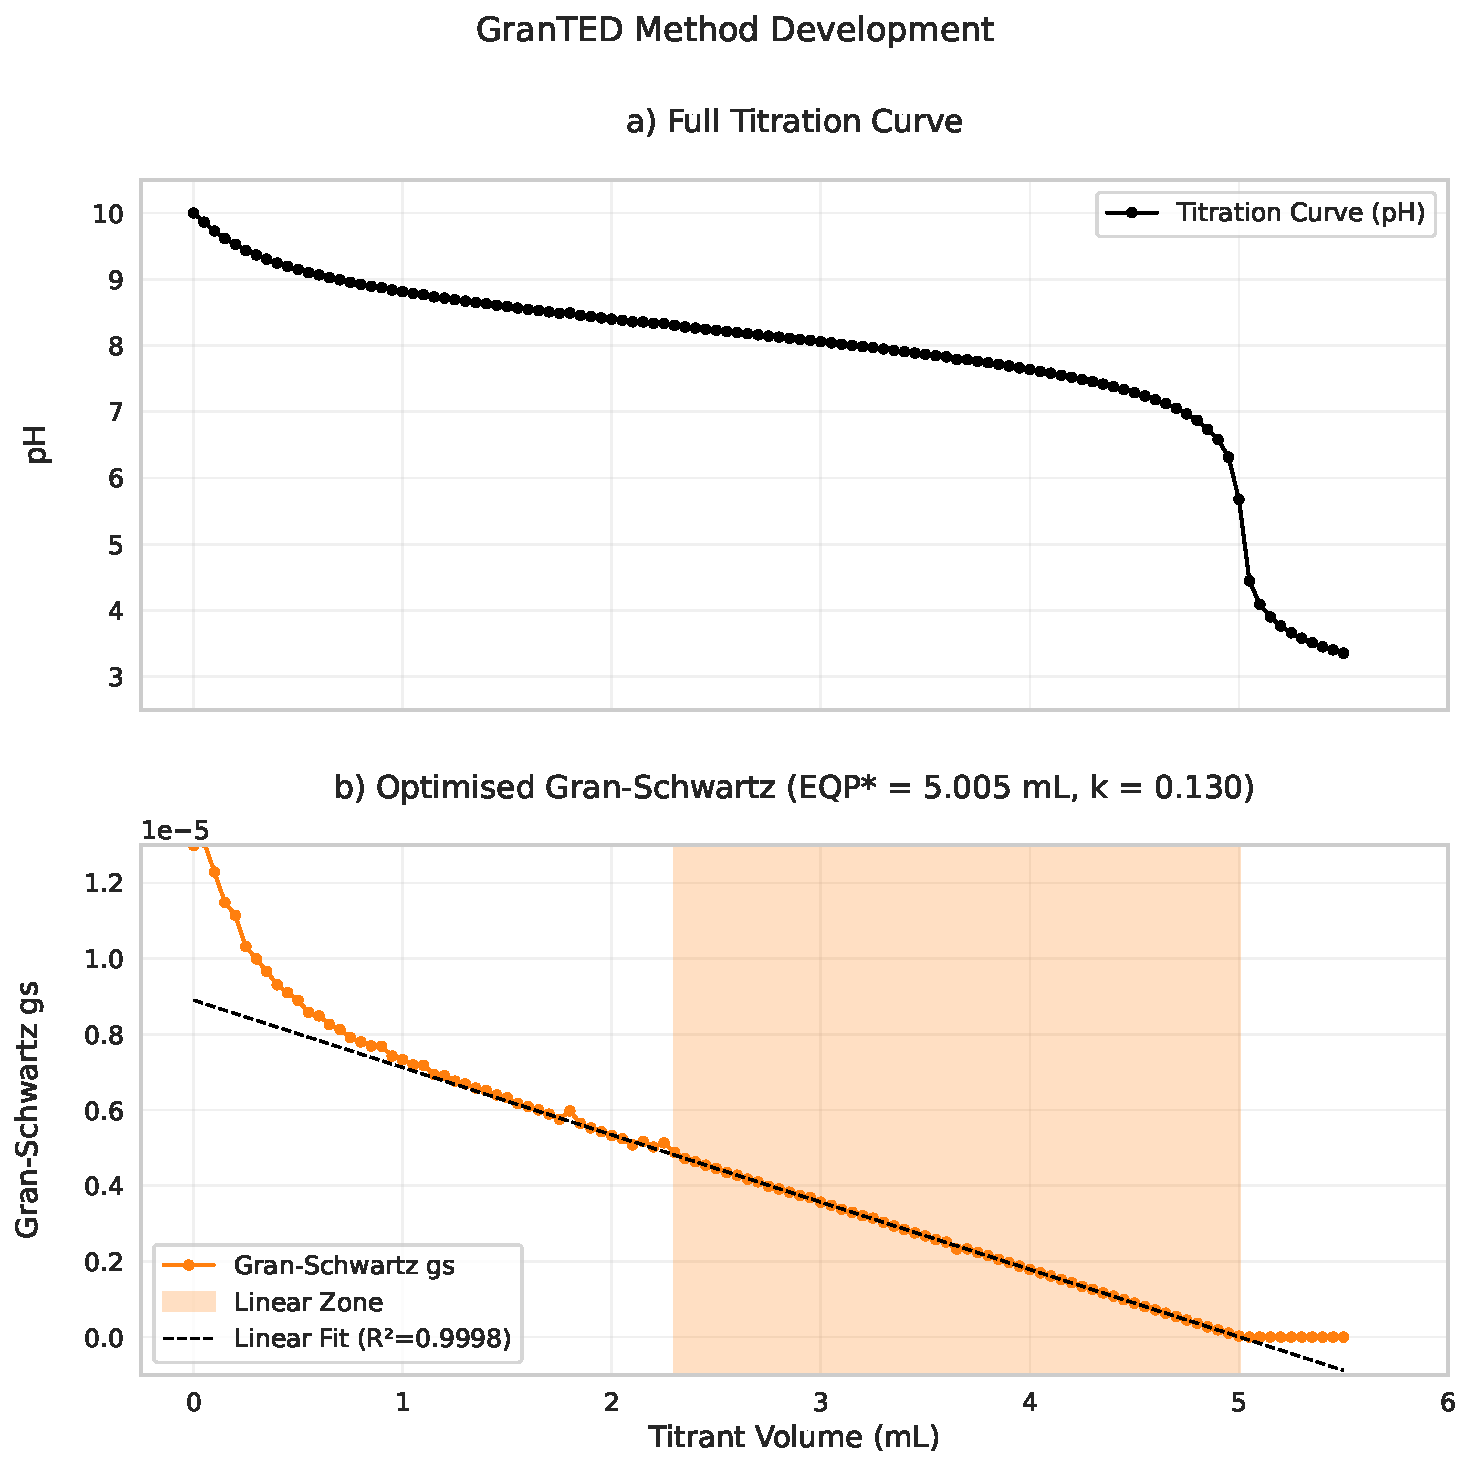
\includegraphics[width=0.48\textwidth]{plots_ab.pdf}
  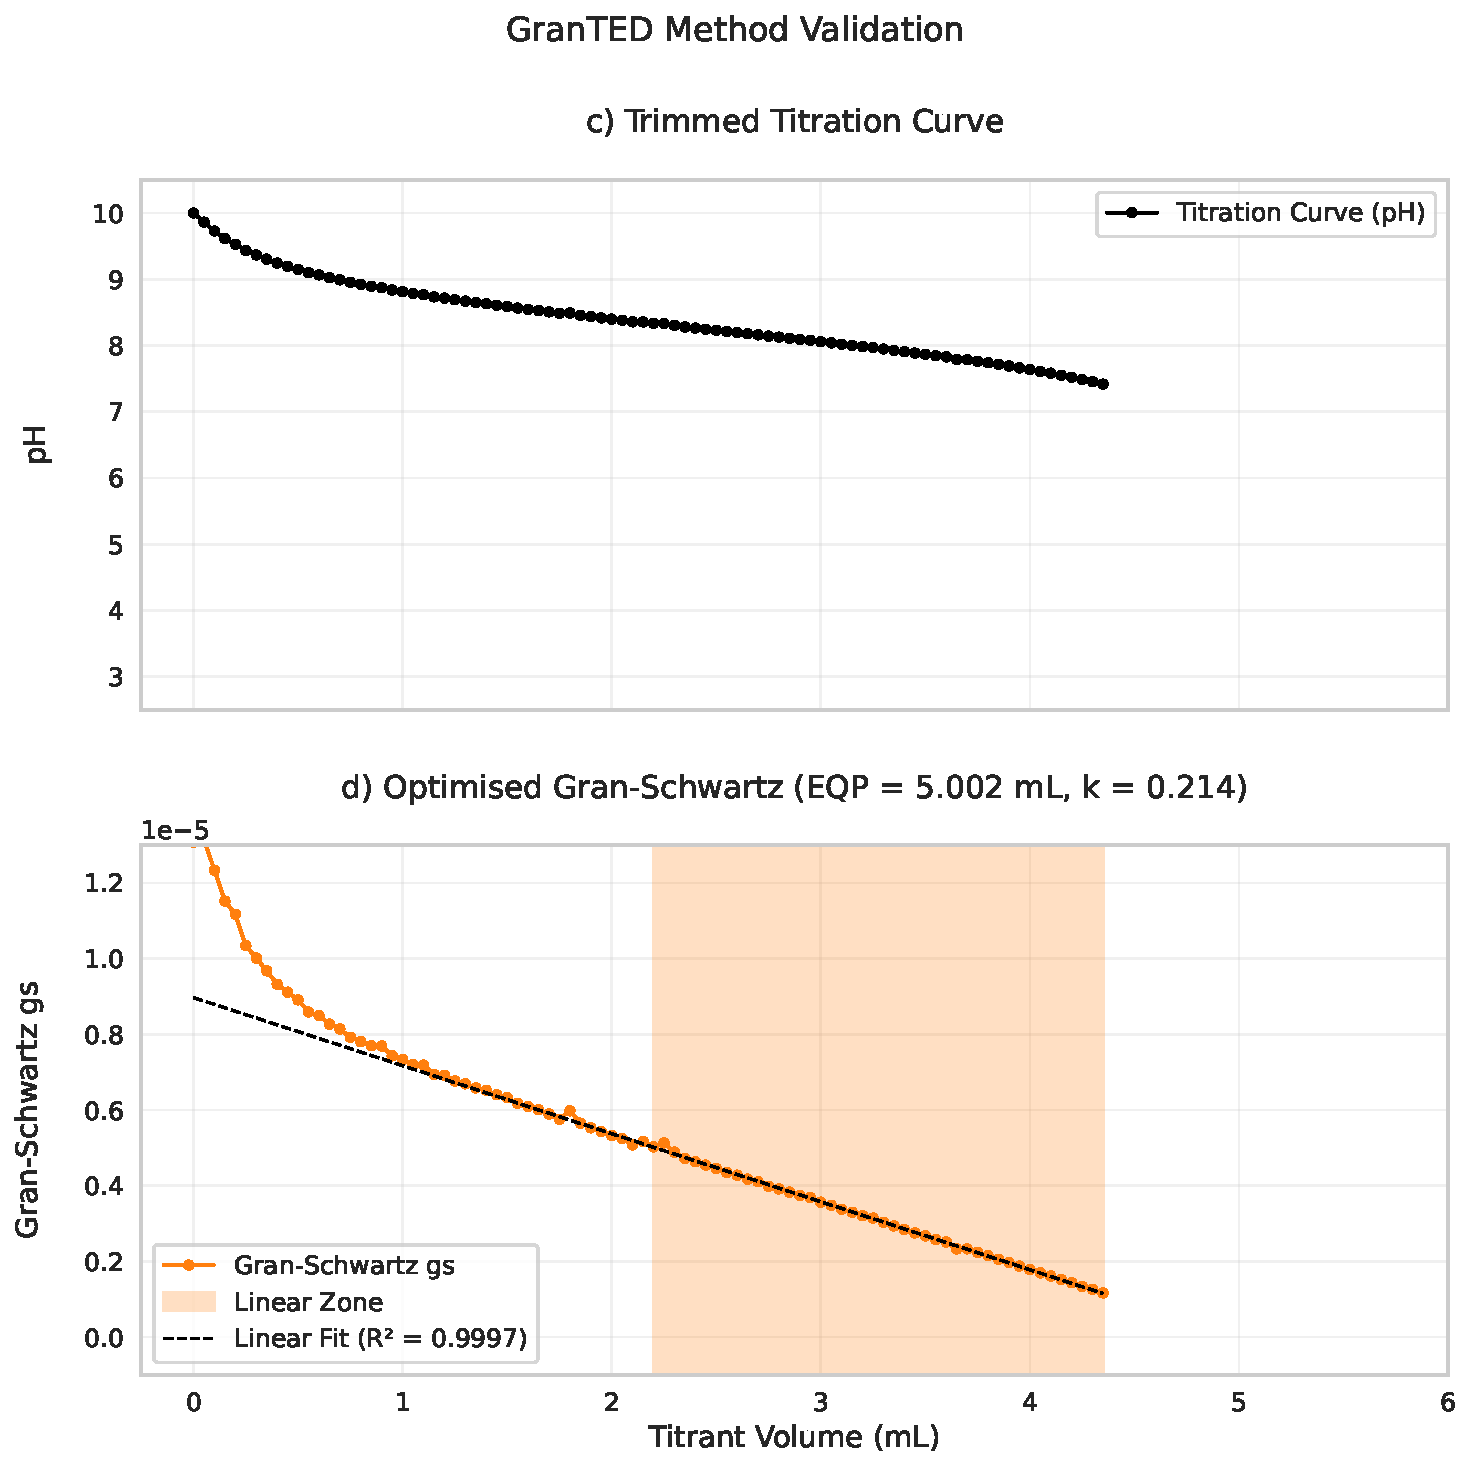
\includegraphics[width=0.48\textwidth]{plots_cd.pdf}
  \caption{Overview of the green analytical strategy for equivalence point (EQP) determination in potentiometric titrations, demonstrated for TRIS (0.1\,M) titrated with \ce{HCl} (0.1\,M).
  Left: a) pH vs. titrant volume ($V$) curve from the initial titration (full run to post-EQP*). %, identifying the pre-EQP linear region (shaded) and its central truncation point (arrow).
  b) Schwartz--Gran modified plot ($V \times 10^{-\mathrm{pH}}$ vs. $V$), showing the straight pre-EQP* line extrapolated to the EQP* (dashed line; intercept at 5.005\,mL).
  Right: c) Titration performed up to the optimal earliest acceptable point volume (4.40\,mL in this case).
  d) Corresponding Schwartz--Green modified plot confirming EQP extrapolation (intercept at 5.002\,mL) with reduced dispensed titrant volume.}
  \label{fig:titrations}
\end{figure*}

\begin{table}[h]
\small
  \caption{Gran--Schwartz results for the \ce{TRIS}/\ce{HCl} system in the vicinity of the optimal volume $V_{\rm opt}$ (4.40\,mL, in bold).
  Full titration EQP* corresponds to 5.005\,mL.
  The selected volume meets the acceptance criteria of deviation from reference EQP* smaller than 0.010\,mL) with excellent linearity and low uncertainty.
  Except for R$^2$, all values in\,mL}
  \label{tab:trimming}
  \begin{tabular*}{0.48\textwidth}{@{\extracolsep{\fill}}lcccc}
    \hline
    Solvent & EQP & Uncertainty & R$^2$ & EQP - EQP* \\
    \hline
    4.25 & 4.980 & 0.010 & 0.9987 & -0.025 \\
    4.30 & 4.987 & 0.010 & 0.9988 & -0.018 \\
    4.35 & 4.989 & 0.009 & 0.9989 & -0.016 \\
    \textbf{4.40} & \textbf{5.002} & \textbf{0.005} & \textbf{0.9997} & \textbf{-0.003} \\
    4.45 & 5.002 & 0.005 & 0.9997 & -0.003 \\
    4.50 & 5.007 & 0.004 & 0.9998 & \phantom{-}0.002 \\
    4.55 & 5.006 & 0.003 & 0.9998 & \phantom{-}0.001 \\
    \hline
  \end{tabular*}
\end{table}

This trimming-based optimisation constitutes the central methodological advance, improving a classical full titration into a reagent-efficient procedure without requiring additional experiments.

\subsection*{Method Validation: Benchmarking against Full Titration}

To validate the accuracy, precision and reliability of the analytical approach, additional titration's Gran--Schwartz equivalence points obtained at the optimised volume \(V_{\rm opt}\) were bench-marked against the same method applied to the full titration.
The conventional inflection-point method applied to the same full titration datasets is also compared.
The inflection-point method relies on the maximum of the first derivative of the S-shaped titration curve for the determination of the equivalence point. This is the main evaluation procedure commonly used in automated titration, but requires titrant consumption well past the equivalence point to accurately capture the steepest slope of the S-shaped curve.

For both benchmark systems \ce{TRIS}/\ce{HCl} and \ce{KHP}/\ce{NaOH}, the equivalence point EQP* determined from the complete dataset of the full curve served as the reference value.
Table~\ref{tab:validation} summarises the results.
In the \ce{TRIS}/\ce{HCl} system, the Gran--Schwartz EQP determined by extrapolation using \(V_{\rm opt}\) agreed with EQP* within the chosen threshold accuracy between 0.010\,mL and 0.050\,mL.
The conventional inflection-point method yielded comparable agreement but only after the full titration volume was reached.
In this case, the EQP corresponds to 5.007 $\pm$ 0.001\,mL.
Similar performance was observed for the \ce{KHP}/\ce{NaOH} system, where the inflection-point EQP corresponds to 5.032 $\pm$ 0.001\,mL.

\begin{table}[h]
\small
  \caption{Comparison between a) EQP*-determination by Gran--Schwartz linear interpolation on the full titration curve, and b) Gran--Schwartz linear extrapolation to determine the EQP. The titration is stopped at the optimal volume \(V_{\rm opt}\) corresponding to the indicated deviation from reference EQP* (see \(V_{\rm opt}\) values in text)
  Results are mean $\pm$ SD ($n=6$ replicates). All values are in\,mL.}
  \label{tab:validation}
  \begin{tabular*}{0.48\textwidth}{@{\extracolsep{\fill}}lcccc}
    \hline
     & a) Reference EQP* & \multicolumn{3}{c}{b) Gran--Schwartz EQP} \\
     &                & \phantom{ $\pm$}0.010 & \phantom{ $\pm$}0.020 & \phantom{ $\pm$}0.050 \\
    \hline
    \multirow{2}{3em}{\ce{TRIS}/\ce{HCl}} & \phantom{ $\pm$}5.003 &  \phantom{ $\pm$}4.990 &  \phantom{ $\pm$}5.005 &  \phantom{ $\pm$}4.992 \\
    & $\pm$ 0.003 & $\pm$ 0.010 & $\pm$ 0.015 & $\pm$ 0.064 \\
    %\hline
    \multirow{2}{3em}{\ce{KHP}/\ce{NaOH}} & \phantom{ $\pm$}5.042 & \phantom{ $\pm$}5.045 & \phantom{ $\pm$}5.051 & \phantom{ $\pm$}5.066 \\
    & $\pm$ 0.003 & $\pm$ 0.003 & $\pm$ 0.015 & $\pm$ 0.041 \\
    \hline
  \end{tabular*}
\end{table}

Importantly, the uncertainty (Table~\ref{tab:trimming}) and the standard deviation (Table~\ref{tab:validation}) associated with the Gran--Schwartz EQP remained low and congruent to the selected difference threshold. % to that of the full method reference EQP*, demonstrating that the early-stop strategy does not compromise precision. 
The comparison of the equivalence points obtained by the three approaches (reference EQP*, Gran--Schwartz EQP at \(V_{\rm opt}\) and conventional inflection point) across both systems confirms excellent consistency.

These results demonstrate that \textsf{GranTED} delivers equivalence points matching analytical quality to the ones provided by the classical inflection-point method, yet systematically achieving them with a substantially reduced reagent consumption.
The automated linear region identification and trimming algorithm eliminates the possible ambiguity inherent in derivative-based analysis while enabling reliable early termination of the titration.

\subsection*{Green Chemistry Metrics and Sustainability Benefits}

The optimised-volume procedure implemented in the analytical strategy directly translates into relevant reductions in titrant consumption.

\(V_{\rm opt}\) identified by the backward trimming procedure strongly depends on the selected accuracy threshold. For the \ce{TRIS}/\ce{HCl} system, \(V_{\rm opt}\) values of 4.4\,mL, 4.3\,mL and 3.6\,mL were obtained at thresholds of 0.010\,mL, 0.020\,mL and 0.050\,mL, respectively.
For the \ce{KHP}/\ce{NaOH} system, the corresponding volumes \(V_{\rm opt}\) were 4.5\,mL, 4.35\,mL and 3.2\,mL.

These substantially reduced values directly lead to significant savings of titrant. For both benchmark systems, the titrant consumption decreased from approximately 10\,\% with 0.010\,mL accuracy threshold to approximately 30\,\% with 0.050\,mL threshold, relative to a conventional full titration continuing well past the equivalence point.

These savings were consistently achieved across both systems, as illustrated in Fig.~\ref{fig:volume_savings} as reagent-saving histogram.

\begin{figure}[h]
\centering
  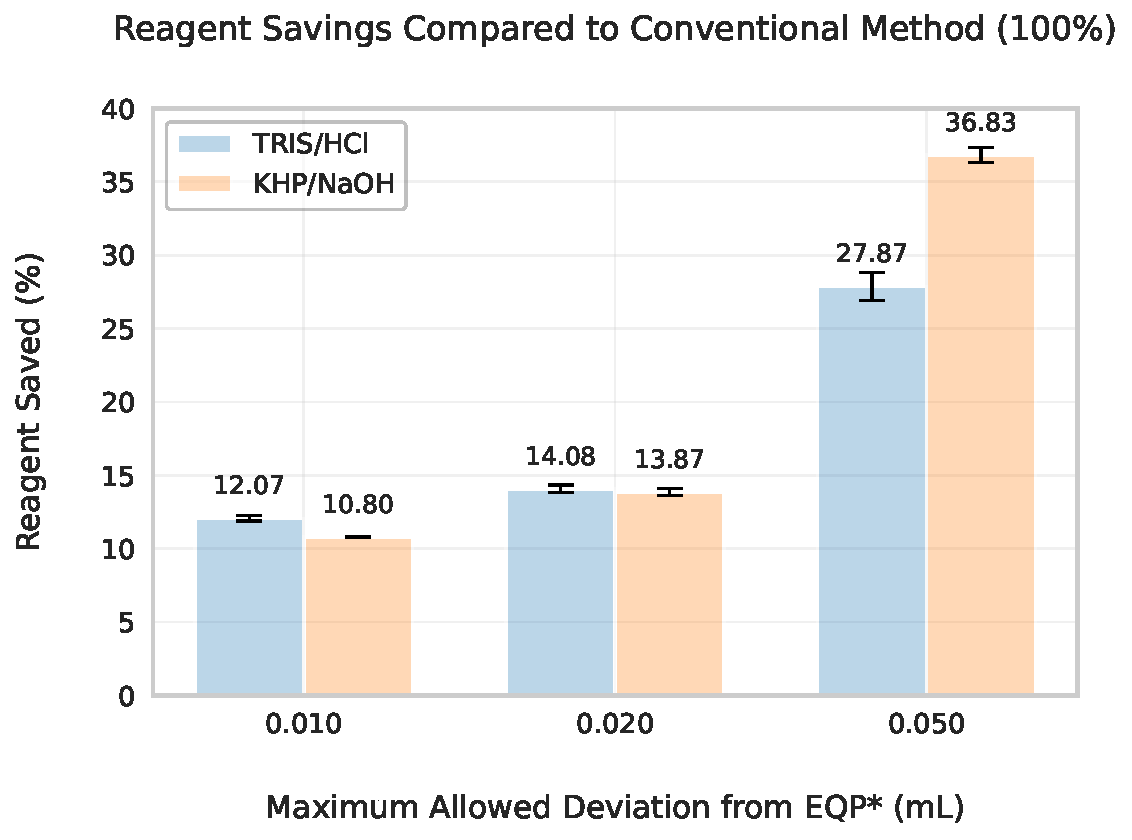
\includegraphics[width=0.48\textwidth]{deviation_histogram.pdf}
  \caption{Reagent savings achieved by stopping at \(V_{\rm opt}\) using different acceptance thresholds (0.010, 0.020 and 0.050\,mL difference from EQP*).
  Results are shown for both \ce{TRIS}/\ce{HCl} and \ce{KHP}/\ce{NaOH} systems ($n=6$ replicates each) and compared against the equivalence point} % and full titration endpoint}
  \label{fig:volume_savings}
\end{figure}

By terminating the titration at the optimised volume \(V_{\rm opt}\), the volume of titrant required is reduced while the determined equivalence point remains within the specified accuracy window.
This allows for reduction of titrant consumption compared to conventional past the equivalence point approach which is needed to reliably identify the inflection point.
For routine laboratories performing multiple replicates or performing high-throughput analyses, this translates into substantial waste minimization.

The demonstrated reagent savings align directly with two core principles of Green Chemistry: Principle 1 (prevention of waste) and Principle 5 (design of safer solvents and auxiliaries).
Reducing titrant consumption lowers both the risk associated to reagents used and the volume of waste generated per analysis.
Furthermore, the open-source nature of \textsf{GranTED} enables widespread adoption in academic and industrial laboratories, promoting more sustainable analytical practices without requiring commercial software.

Overall, the analytical strategy \textsf{GranTED} demonstrates that modern computational linerarisation combined with systematic data trimming can transform a classical analytical method into a greener, more efficient procedure while maintaining high analytical performance.

\section*{Conclusions}

We have introduced a new, green analytical strategy developed within \textsf{GranTED}, an open-source Python toolkit that implements a two-stage Gran--Schwartz linerarisation strategy for potentiometric titrations.
By combining a full titration to establish a reference equivalence point (EQP*) with systematic backward trimming, the software reliably identifies the earliest acceptable volume \(V_{\rm opt}\) at which the Gran--Schwartz equivalence point (EQP) converges within a user-defined accuracy threshold (typically 0.010--0.050\,mL). 

Applied to the benchmark systems \ce{TRIS}/\ce{HCl} and \ce{KHP}/\ce{NaOH}, this approach consistently delivered equivalence points in excellent agreement with both the reference EQP* and the conventional inflection-point method, while reducing titrant consumption by about 10--30\,\% for each single titration.
The strategy requires no additional experiments or hardware and eliminates the subjectivity associated with manual selection of the linear region.

\textsf{GranTED} therefore provides a practical, accurate, precise and greener alternative to traditional potentiometric titration workflows.
By enabling earlier termination of titrations without loss of analytical quality, it directly supports Green Chemistry Principle 1 (prevention of waste) and Principle 5 (design of safer solvents and auxiliaries).
As a freely available, MIT-licensed tool with comprehensive diagnostic and visualisation capabilities, \textsf{GranTED} may find wide application in research, quality control, and teaching laboratories seeking more sustainable analytical practices.

Furthermore, similar tunable criteria-based approach, open the possibility for an {\it online, direct forward method} in which the titration is automatically terminated on-the-fly, during the titration itself, in a sample-driven manner, as soon as the Gran--Schwartz linear fit results satisfy the defined thresholds (e.g. EQP evolution, standard error or R$^2$) convergence.

Future extensions will include support for complexometric, precipitation, and redox titrations, as well as the analysis of polyprotic substances for additional green analytical workflows.

\section*{Author Contributions}

S.G. and C.A.D.C. conceptualised the study, developed the methodology, performed the investigation and formal analysis, curated the data, visualised the results, and wrote the original draft.% S.G. developed the software. C.A.D.C. carried out the experiments.

\section*{Conflicts of Interest}

S.G. declares no conflicts of interest. C.A.D.C. is currently working for a manufacturer of laboratory analytical instrumentation (Mettler-Toledo Technologies GmbH).

\section*{Acknowledgments}

The authors gratefully acknowledge Dr.~Mohammad Torabi Dashti for fruitful discussions and valuable suggestions.

\section*{Data Availability}

The datasets supporting this article are available at \href{https://github.com/sgiani95/GranTED/}{\texttt{https://github.com/sgiani95/GranTED/}} or from the corresponding authors upon reasonable request.

%%%REFERENCES%%%


\bibliography{rsc} %You need to replace "rsc" on this line with the name of your .bib file
\bibliographystyle{rsc} %the RSC's .bst file




\end{document}